\documentclass{article}
\usepackage{boxedminipage}
\usepackage{color}
\usepackage{amsmath}
\usepackage{amssymb}
\usepackage{amsthm}
\usepackage{bm}
\usepackage{xy}
\usepackage{geometry}
\usepackage{fullpage}
\usepackage{graphicx}
\usepackage{float}
\usepackage{url}            %for \url{www.---} in bibliography
\DeclareGraphicsExtensions{.png}

\title{Stuff with spectrums}
\author{Ryan Holmes} \geometry{a4paper}

\begin{document}
\maketitle
\section{Single sided amplitude spectrum}

A single sided amplitude spectrum is calculated in AmpSpec.m An
example calculation on the signal:
\begin{align*}
x &= 0:0.01:2000 \\
S &= \sin{2\pi x/10}+0.5\sin{2\pi x/10}+2\sin{2\pi x/200} \end{align*}

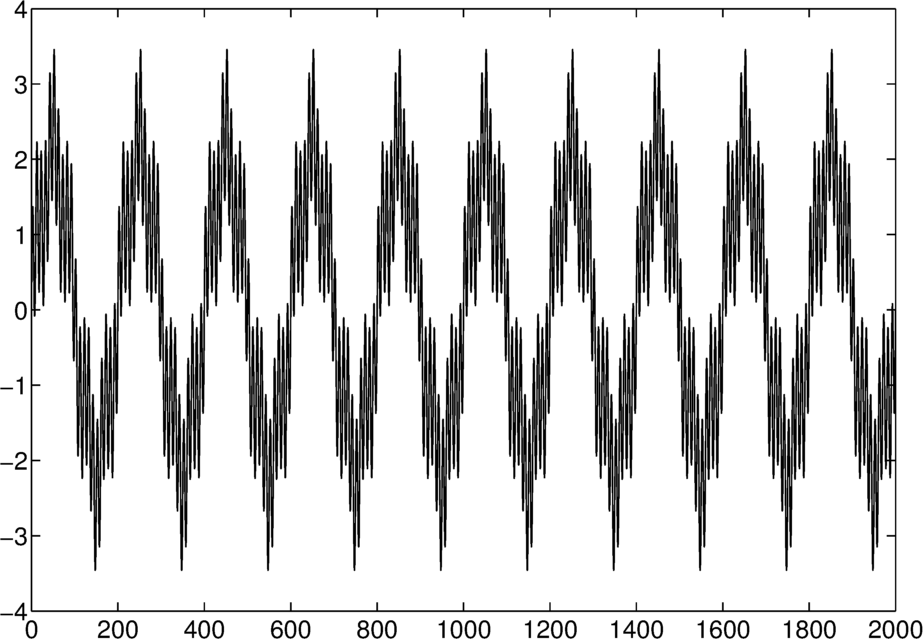
\includegraphics[width=8cm]{signalplot.png}

without a Hamming window the resulting one-sided amplitude spectrum
is

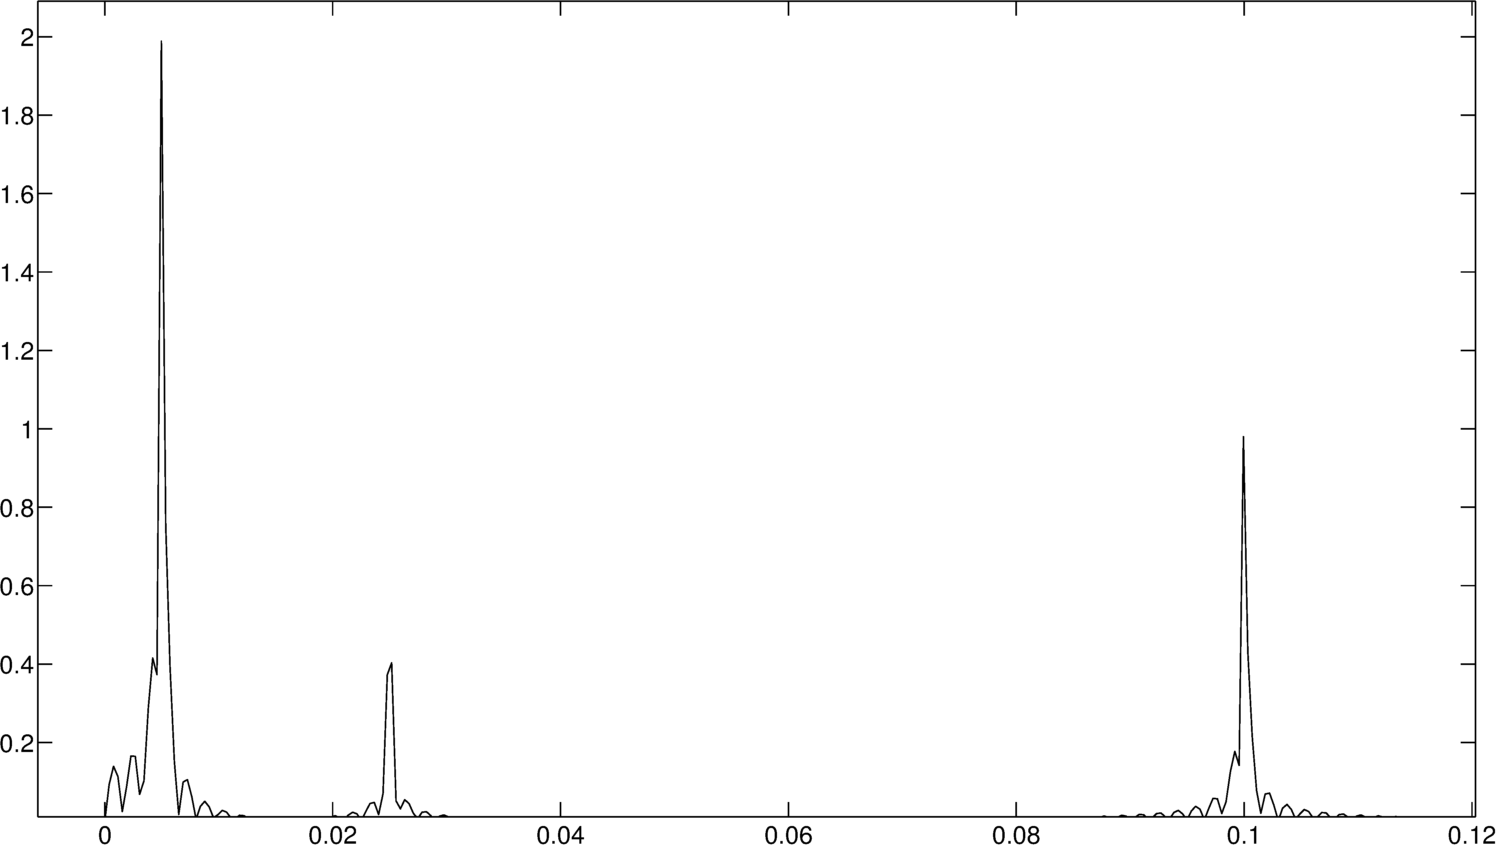
\includegraphics[width=8cm]{AmpSpecNoHam.png}

Note that the amplitudes of the peaks approach the amplitudes of the
sin waves at 1, 0.5 and 2.
If we include a hamming window without doing any amplitude correction
then we get.
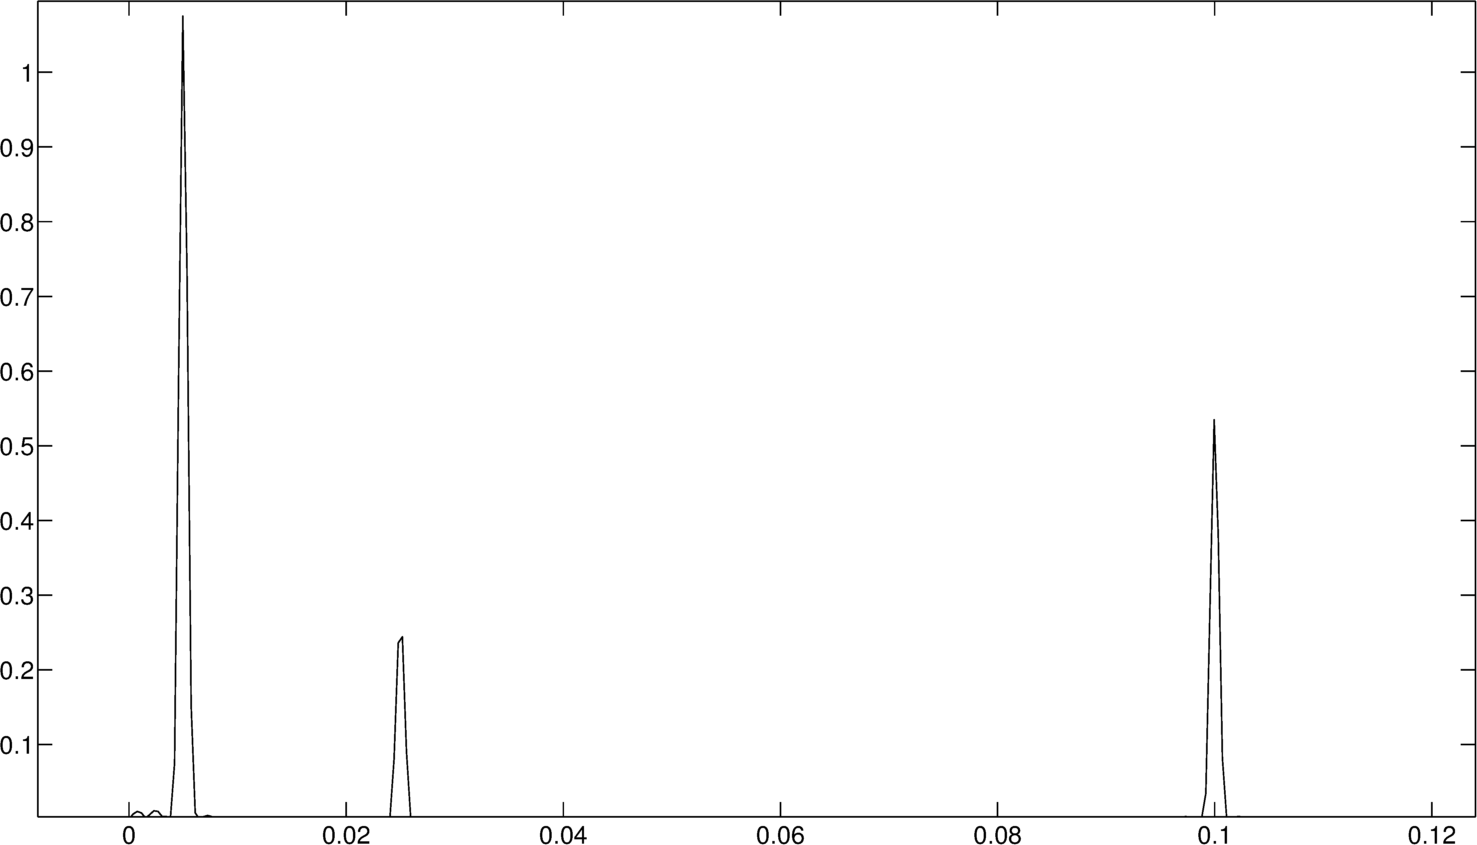
\includegraphics[width=8cm]{AmpSpecHam.png}

Note that the side lobes have dissapeared but that the peak amplitudes
have reduced. This is because the hamming window (which multiplies in
the time domain) reduces the power of the signals by a constant
amount. To correct, we multiply the spectrum by the amplitude
correction factor being 1.855 for the hamming window. The result has
peaks that approch the correct amplitude but without the side lobes.

\section{Spectral Integral}
The function periodiogram and bandpower can be used for this.

\section{Discrete Fast Fourier Transform}
The DFT on a signal of length $N$ is defined as:
\begin{equation} X_k = \sum_{j=0}^{N-1} x_j e^{-\frac{2\pi i j }{N}k} \end{equation}
Here the argument of the exponential runs from $j/N=0$ to $j/N=N-1/N$,
and thus each value of $k$ represents a sinusoid of period
$T=\frac{2\pi}{\omega} = \frac{1}{k}$ on the domain $j/N=[0,1)$. To
get the inverse transform, we multiply by another sinusoid and sum
over $k$:
\begin{align} \sum_{k=0}^{N-1} X_k e^{\frac{2\pi i k}{N}m} &=
  \sum_{k=0}^{N-1}\sum_{j=0}^{N-1} x_j e^{-\frac{2\pi i j
    }{N}k}e^{\frac{2\pi i k}{N}m}
\\ &= \sum_{j=0}^{N-1} x_j \left(\sum_{k=0}^{N-1}e^{-\frac{2\pi i j
    }{N}(k-m)}\right) \\
&= \sum_{j=0}^{N-1} x_j \left(N\delta_{km}\right)\\
\Longrightarrow x_m &= \sum_{k=0}^{N-1} \frac{X_k}{N} e^{\frac{2\pi i
    k}{N}m}
\end{align}

Thus we see that the original signal $x_j$ is now expressed as a sum
of sinusoids with amplitude $|X_k|/N$ and phase $arg(X_k)$.

\end{document}